\documentclass[10pt]{article}
\usepackage[T1]{fontenc}

% Document Details
\newcommand{\CLASS}{AMATH 563}
\newcommand{\assigmentnum}{Nueral Networks}

\usepackage[margin = 1in, left=0.75in,right=0.75in]{geometry}
\usepackage{titling}
\setlength{\droptitle}{-6em}   % This is your set screw
\date{}
\renewcommand{\maketitle}{
	\clearpage
	\begingroup  
	\centering
	\LARGE \sffamily\textbf{\CLASS} \Large \assigmentnum\\[.8em]
	\large Tyler Chen\\[1em]
	\endgroup
	\thispagestyle{empty}
}
 % Title Styling


\usepackage{enumitem}

% Figures
\usepackage{subcaption}

% TikZ and Graphics
\usepackage{tikz, pgfplots}
\pgfplotsset{compat=1.12}
\usetikzlibrary{patterns,arrows}
\usepgfplotslibrary{fillbetween}

\usepackage{pdfpages}
\usepackage{adjustbox}

\usepackage{lscape}
\usepackage{titling}
\usepackage[]{hyperref}


% Header Styling
\usepackage{fancyhdr}
\pagestyle{fancy}
\lhead{\sffamily \CLASS}
\rhead{\sffamily Chen \textbf{\thepage}}
\cfoot{}

% Paragraph Styling
\setlength{\columnsep}{1cm}
\setlength{\parindent}{0pt}
\setlength{\parskip}{5pt}
\renewcommand{\baselinestretch}{1}

% TOC Styling
\usepackage{tocloft}
\iffalse
\renewcommand{\cftsecleader}{\cftdotfill{\cftdotsep}}

\renewcommand\cftchapafterpnum{\vskip6pt}
\renewcommand\cftsecafterpnum{\vskip10pt}
\renewcommand\cftsubsecafterpnum{\vskip6pt}

% Adjust sectional unit title fonts in ToC
\renewcommand{\cftchapfont}{\sffamily}
\renewcommand{\cftsecfont}{\bfseries\sffamily}
\renewcommand{\cftsecnumwidth}{2em}
\renewcommand{\cftsubsecfont}{\sffamily}
\renewcommand{\cfttoctitlefont}{\hfill\bfseries\sffamily\MakeUppercase}
\renewcommand{\cftaftertoctitle}{\hfill}

\renewcommand{\cftchappagefont}{\sffamily}
\renewcommand{\cftsecpagefont}{\bfseries\sffamily}
\renewcommand{\cftsubsecpagefont}{\sffamily}
\fi
 % General Styling
% Code Display Setup
\usepackage{listings,lstautogobble}
\usepackage{lipsum}
\usepackage{courier}
\usepackage{catchfilebetweentags}

\lstset{
	basicstyle=\small\ttfamily,
	breaklines=true, 
	frame = single,
	rangeprefix=,
	rangesuffix=,
	includerangemarker=false,
	autogobble = true
}


\usepackage{algorithmicx}
\usepackage{algpseudocode}

\newcommand{\To}{\textbf{to}~}
\newcommand{\DownTo}{\textbf{downto}~}
\renewcommand{\algorithmicdo}{\hspace{-.2em}\textbf{:}}
 % Code Display Setup
% AMS MATH Styling
\usepackage{amsmath, amssymb}
\newcommand{\qed}{\hfill\(\square\)}

%\newtheorem*{lemma}{Lemma} 
%\newtheorem*{theorem}{Theorem}
%\newtheorem*{definition}{Definition}
%\newtheorem*{prop}{Proposition}
%\renewenvironment{proof}{{\bfseries Proof.}}{}


% mathcal
\newcommand{\cA}{\ensuremath{\mathcal{A}}}
\newcommand{\cB}{\ensuremath{\mathcal{B}}}
\newcommand{\cC}{\ensuremath{\mathcal{C}}}
\newcommand{\cD}{\ensuremath{\mathcal{D}}}
\newcommand{\cE}{\ensuremath{\mathcal{E}}}
\newcommand{\cF}{\ensuremath{\mathcal{F}}}
\newcommand{\cG}{\ensuremath{\mathcal{G}}}
\newcommand{\cH}{\ensuremath{\mathcal{H}}}
\newcommand{\cI}{\ensuremath{\mathcal{I}}}
\newcommand{\cJ}{\ensuremath{\mathcal{J}}}
\newcommand{\cK}{\ensuremath{\mathcal{K}}}
\newcommand{\cL}{\ensuremath{\mathcal{L}}}
\newcommand{\cM}{\ensuremath{\mathcal{M}}}
\newcommand{\cN}{\ensuremath{\mathcal{N}}}
\newcommand{\cO}{\ensuremath{\mathcal{O}}}
\newcommand{\cP}{\ensuremath{\mathcal{P}}}
\newcommand{\cQ}{\ensuremath{\mathcal{Q}}}
\newcommand{\cR}{\ensuremath{\mathcal{R}}}
\newcommand{\cS}{\ensuremath{\mathcal{S}}}
\newcommand{\cT}{\ensuremath{\mathcal{T}}}
\newcommand{\cU}{\ensuremath{\mathcal{U}}}
\newcommand{\cV}{\ensuremath{\mathcal{V}}}
\newcommand{\cW}{\ensuremath{\mathcal{W}}}
\newcommand{\cX}{\ensuremath{\mathcal{X}}}
\newcommand{\cY}{\ensuremath{\mathcal{Y}}}
\newcommand{\cZ}{\ensuremath{\mathcal{Z}}}

% mathbb
\usepackage{bbm}
\newcommand{\bOne}{\ensuremath{\mathbbm{1}}}

\newcommand{\bA}{\ensuremath{\mathbb{A}}}
\newcommand{\bB}{\ensuremath{\mathbb{B}}}
\newcommand{\bC}{\ensuremath{\mathbb{C}}}
\newcommand{\bD}{\ensuremath{\mathbb{D}}}
\newcommand{\bE}{\ensuremath{\mathbb{E}}}
\newcommand{\bF}{\ensuremath{\mathbb{F}}}
\newcommand{\bG}{\ensuremath{\mathbb{G}}}
\newcommand{\bH}{\ensuremath{\mathbb{H}}}
\newcommand{\bI}{\ensuremath{\mathbb{I}}}
\newcommand{\bJ}{\ensuremath{\mathbb{J}}}
\newcommand{\bK}{\ensuremath{\mathbb{K}}}
\newcommand{\bL}{\ensuremath{\mathbb{L}}}
\newcommand{\bM}{\ensuremath{\mathbb{M}}}
\newcommand{\bN}{\ensuremath{\mathbb{N}}}
\newcommand{\bO}{\ensuremath{\mathbb{O}}}
\newcommand{\bP}{\ensuremath{\mathbb{P}}}
\newcommand{\bQ}{\ensuremath{\mathbb{Q}}}
\newcommand{\bR}{\ensuremath{\mathbb{R}}}
\newcommand{\bS}{\ensuremath{\mathbb{S}}}
\newcommand{\bT}{\ensuremath{\mathbb{T}}}
\newcommand{\bU}{\ensuremath{\mathbb{U}}}
\newcommand{\bV}{\ensuremath{\mathbb{V}}}
\newcommand{\bW}{\ensuremath{\mathbb{W}}}
\newcommand{\bX}{\ensuremath{\mathbb{X}}}
\newcommand{\bY}{\ensuremath{\mathbb{Y}}}
\newcommand{\bZ}{\ensuremath{\mathbb{Z}}}

% alternative mathbb
\newcommand{\NN}{\ensuremath{\mathbb{N}}}
\newcommand{\RR}{\ensuremath{\mathbb{R}}}
\newcommand{\CC}{\ensuremath{\mathbb{C}}}
\newcommand{\ZZ}{\ensuremath{\mathbb{Z}}}
\newcommand{\EE}{\ensuremath{\mathbb{E}}}
\newcommand{\PP}{\ensuremath{\mathbb{P}}}
\newcommand{\VV}{\ensuremath{\mathbb{V}}}
\newcommand{\cov}{\ensuremath{\text{Co}\VV}}
% Math Commands

\newcommand{\st}{~\big|~}
\newcommand{\stt}{\text{ st. }}
\newcommand{\ift}{\text{ if }}
\newcommand{\thent}{\text{ then }}
\newcommand{\owt}{\text{ otherwise }}

\newcommand{\norm}[1]{\left\lVert#1\right\rVert}
\newcommand{\snorm}[1]{\lVert#1\rVert}
\newcommand{\ip}[1]{\ensuremath{\left\langle #1 \right\rangle}}
\newcommand{\pp}[3][]{\frac{\partial^{#1}#2}{\partial #3^{#1}}}
\newcommand{\dd}[3][]{\frac{\d^{#1}#2}{\d #3^{#1}}}
\renewcommand{\d}{\ensuremath{\mathrm{d}}}

\newcommand{\indep}{\rotatebox[origin=c]{90}{$\models$}}




 % Math shortcuts

\usepackage{dblfloatfix}    % To enable figures at the bottom of page

% Problem
\newenvironment{problem}[1]{\vspace{2em}{\large\sffamily\textbf{#1}}\itshape\par}{}

\usepackage{nameref}
\newcommand{\vln}{\rotatebox{90}{--}}

\begin{document}

\twocolumn[{%
\begin{@twocolumnfalse}
\maketitle
\vspace{2em}
\begin{abstract}
We outline a how neural networks might be applied to the study of systems governed by possibly unknown PDEs. In particular we show that future state predictions are possible for some systems, even if they are chaotic. We address how high dimensional data can be rank reduced first in order to allow for training on a smaller neural net. While some results are encouraging, we find that it is quite difficult to correctly tune the neural networks in a limited time.
\end{abstract}

\vspace{4em}
%\tableofcontents
%\vspace{3em}
\pagebreak\end{@twocolumnfalse}
}]

\section{Introduction and Overview}
With recent increases in computation power and data storage capabilities our ability effectively process data computationally has increases substantially. Machine learning uses statistical techniques to gather information about a dataset and use it to make predictions or understand trends. One class of machine learning methods, neural networks, is particularly effective given large datasets. If neural nets can be effectively used to predict solutions of PDEs then we can step away from trying to guess at the PDEs which actually describe systems and move towards generating trajectories using these neural nets.

\section{Theoretical Background}
\subsection{Neural Network Basics}
Suppose we have sets \( \hat{X}_0 \) and \( \hat{X}_N \) with elements of size \( m \) and \( n \) respectively. Let \( \hat{f}:\hat{X}_0 \to \hat{X}_N \) be an injection. The goal of a neural network is to be able to accurately compute this injection to make predictions about elements of \( \hat{X}_0 \) for which we do not know the actual value of \( \hat{f} \).

A feed forward neural network is a function of the form,
\begin{align}
    X_N = f_N(b_{N-1}+\cdots f_2(b_1+ W_1f_1(b_0 + W_0x_0))) \label{NN}
\end{align}
where the the ``activation'' functions \( f_j:\RR\to\RR \) are applied componentwise.

Each ``layer'' is of the form,
\begin{align*}
    x_{j+1} = f_{j+1}j(W_j x_{j} + b_j), && j=0,1,\ldots, N-1
\end{align*}

Note that \( W_j \) can be of any shape compatible with \( x_j \) with the constraint that \( W_{N-1} \) must also give something of the dimension of \( x_N \).

The goal is to set the parameters \( W_j \) and \( b_j \) so that the neural network is equal to \( \hat{f} \). However, it is clear that unless we know the output of \( f \) on all of \( \hat{X}_0 \) this will not be possible even if our neural net has the same form as \( \hat{f} \). Since in general we would like to be able to make predictions about unknown data we will have to settle for the neural network being an approximation to \( \hat{f} \).

More specifically, let \( X_0\subset \hat{X}_0 \) and suppose the value of \( \hat{f}(x) \) is known for all \( x\in X_0 \). For convenience we will write \( X_0 \) as a matrix of size \( n\times t \). Define \( X_N\subset \hat{X}_N \) as the \( m\times t \) matrix found by applying \( \hat{f} \) to the columns of \( X_0 \). We will use the data from \( X_0 \) to train the neural net to (hopefully) give us a good approximation for \( \hat{f} \). Since the neural network can take any element of \( \hat{X}_0 \) as input, we hope that it can be used for predictions about the value of \( \hat{f} \) on these elements.


\subsection{Loss functions}
Given a neural network we would like to train it to be able to make predictions. In order to do this we need some way of saying what a good prediction is. In general this is done by defining a loss function which is small when the network gives good predictions, and large when it gives bad predictions.

More specifically, let \( X_0\in\RR^{n} \) and \( X_N\in\RR^{m} \) be the input data and target data respectively. Let \( f:\RR^{n}\times\RR^{Z}\to\RR^{m} \) be a neural network as defined above, where \( Z \) is the number of free parameters. The residual error of the network for a fixed set of parameters \( \beta\in\RR^{Z} \) is \( Y - f(X,\beta) \).

Ideally the residual error is zero. By picking some metric with which to measure the residual error, we have a minimization problem. In this paper we often chose to minimize the mean square error, which amounts to solving,
\begin{align}
    \min_{\beta} \sum_{x_0\in X_0} \norm{\hat{f}(x_0)-f(x_0,\beta)}_2^2 \label{mse}
\end{align}

\subsection{Optimizers}
In order to minimize expressions such as (\ref{mse}) an optimization algorithm must be applied. Since the input and output lie in such high dimensional spaces, the loss function often has many local minimum or saddle points. As such, traditional methods such as gradient decent may not work very well. Instead there are many popular gradient based algorithms which introduce some stochasticity in order to avoid ``getting stuck''. Since our neural network can be expressed as the composition of fairly straightforward functions, the gradient with respect to entries of \( \beta \) can be easily computed using the chain rule (done by something called back-propagation).

\subsection{SVD and Data reduction}
When training a neural network the size of the input and output are determine by the data given. This means the network may have to be very large the the beginning and end nodes. On approach to reduce the size of the network is to project the input and target data into lower dimensional subspaces and then train on the projections. This is equivalent to the first and last hidden layers of the neural net being of smaller size and with fixed weights. If the weights are not fixed, the net will determine the ``best'' projection. However, since the SVD already computes the optimal low rank approximation in the 2-norm or Frobenius norm, it may be beneficial to set these weights so that the net does not have to learn them.

Suppose our input data \( X \) is in \( \RR^{N} \) and we have \( T \) samples. We then have a \( N\times T \) data matrix. We would like to find a subspace of \( \RR^{N} \) of lower dimension where our data can be approximated well. Our data has a rank \( k \) reduced SVD,
\begin{align}
    X \approx U\Sigma V^* \label{SVD_eq}
\end{align}
where \( U  \) is \( N\times k \), \( \Sigma \) is \( k\times k \), and \( V^* \) is \( k\times T \). We interpret this in the following way: the columns of \( U \) are the dominant modes in our data, and the rows of \( \Sigma V^* \) tell us how these modes vary in time. We can therefore use the columns of \( \Sigma V^* \), which are of height \( k \), as our approximation to the input data.

In general the input and target data will not be of the same size or, for time series data, of the same dynamics. However, in the case that they are the rank reduction used on the input and output can be computed simultaneously saving a large computation. While it will no longer be the optimal reduction for each of these, it will be near optimal. In this paper we are generally building steppers, and so the input and target are of the same system at different times. We therefore compute the low dimensional spaces by taking the SVD of the full data set, and then split it into the input and target data sets.

\section{Algorithm Implementation and Development}

\subsection{Neural Network Framework}
We use the python libraries Keras and Tensorflow for most of our neural nets. In addition the neural network package for MATLAB is occasionally used.

In general, the setup and labeling of the data was the primary focus of this project. It is straightforward to change the net structure and tune other hyperparameters once this has been done. However, doing so is time consuming. If any of the nets work at all this should be taken as very encouraging since they were generally chosen at random without much justification.


\subsection{Data Generation}
To generate data for our systems we generally use an ODE stepper to solve a system of ODEs corresponding to the discrimination of a PDE. The target data is taken to be the training data one step forward in time (with respect to some fixed time mesh). Multiple initial conditions are generated in a variety of ways depending on


\subsection{Kuramoto-Sivashinsky Equation}
We are provided with a stepper to produce solutions to the Kuramoto-Sivashinsky equation (\ref{KS_eqn}) with periodic boundary conditions on a given mesh (with \( N \) spatial points and \( T \) time points).
\begin{align}
    \pp{u}{t} = -u \pp{u}{x} - \pp[2]{u}{x} - \pp[4]{u}{x} \label{KS_eqn}
\end{align}

In order to train our network to step forward in time we must generate a batch of trajectories stemming from some class of initial conditions. To do this we start with a zero initial condition and then randomly set a fixed (generally two or three) number Fourier modes to have weights with real and imaginary parts uniformly distributed on \( [-N/2,N/2] \). This produces periodic initial conditions which lead to fairly nice behavior. We then generate a solutions with these initial conditions and save them.

The data is then imported to Python and formatted into the training and target data sets by appropriate slicing. A neural net defined in Keras is trained to predict the value of \( u(t+\Delta t) \) given the value of \( u(t) \).

\begin{figure}[t]\centering
\begin{subfigure}{.45\textwidth}\centering
    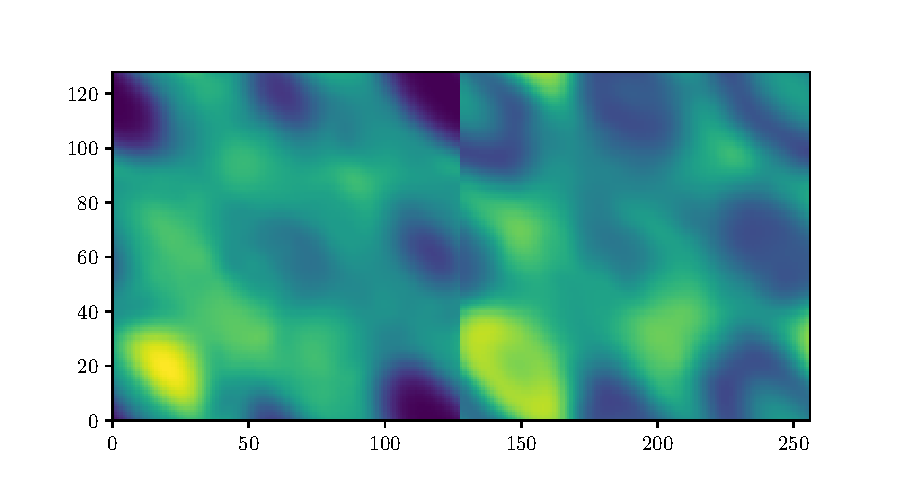
\includegraphics[width=\textwidth]{img/svd_mode_1.pdf}
    \caption{1st left singular vector reshaped}
    \label{1mode}
\end{subfigure}\hfill
\begin{subfigure}{.45\textwidth}\centering
    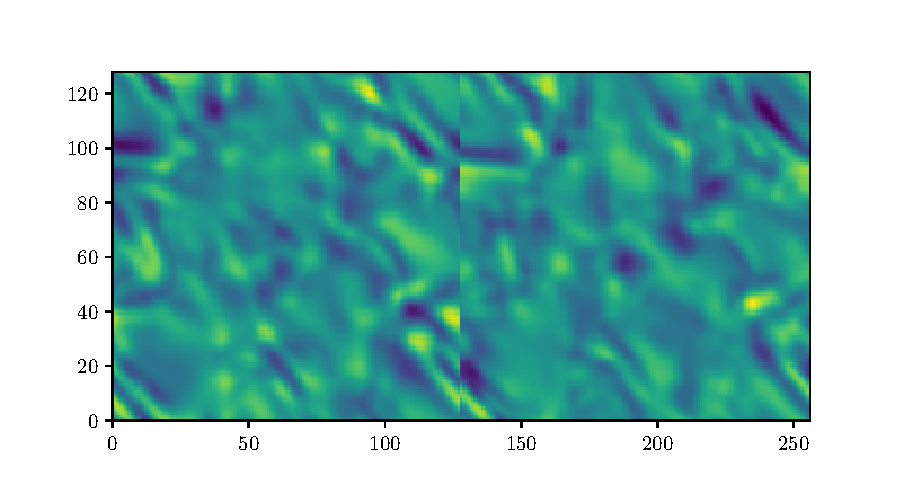
\includegraphics[width=\textwidth]{img/svd_mode_100.pdf}
    \caption{100th singular vector reshaped}
    \label{100mode}
\end{subfigure}
\caption{SVD modes for \( u \) (left) and \( v \) (right) }
\label{SVD_modes}
\end{figure}

\begin{figure}[t]\centering
\begin{subfigure}{.45\textwidth}\centering
    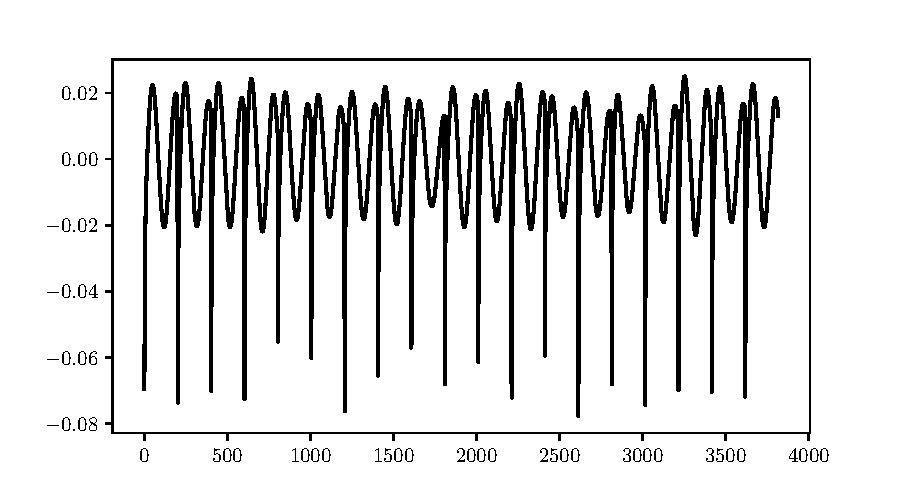
\includegraphics[width=\textwidth]{img/svd_coeff_1.pdf}
    \caption{1st right singular vector varying in time}
    \label{1coeff}
\end{subfigure}
\begin{subfigure}{.45\textwidth}\centering
    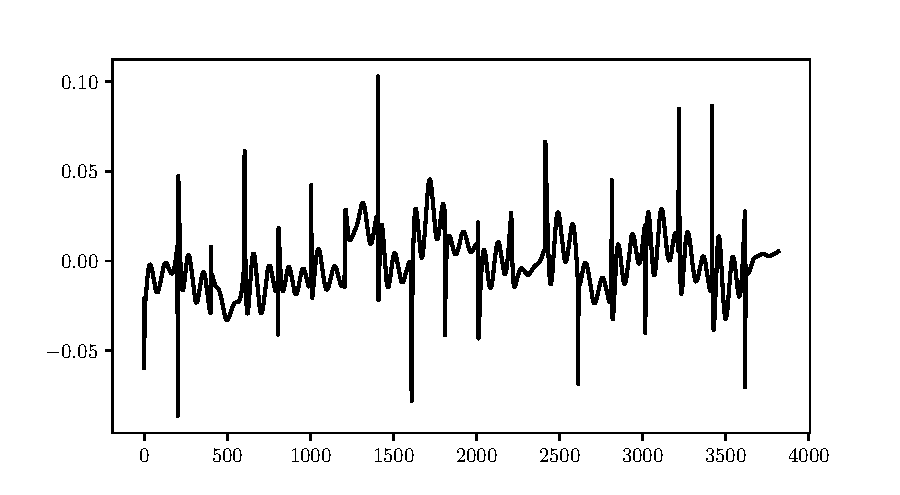
\includegraphics[width=\textwidth]{img/svd_coeff_100.pdf}
    \caption{100th right singular vector varying in time}
    \label{100coeff}
\end{subfigure}
\caption{coefficients of SVD modes vs dataset}
\label{SVD_coeff}
\end{figure}

\subsection{ \( \boldsymbol\lambda \)-\( \boldsymbol\omega \) Reaction-Diffusion Equation}
We can apply similar methods to a PDE in two dimensions.
With,
\begin{align*}
    {\bf u} = \left[\begin{array}{c}u \\ v\end{array}\right], &&
    {\bf D} = \left[\begin{array}{cc}d_1 \\ & d_2 \end{array}\right]
\end{align*}
the Kuramoto-Sivashinsky equation is defined as,
\begin{align}
    \pp{{\bf u}}{t} =
    \left[\begin{array}{cc}
        \lambda(s) & -\omega(s) \\
        \omega(s) & \lambda(s)
    \end{array}\right]
    {\bf u}
    + {\bf D} \nabla^2 {\bf u} \label{RD_eqn}
\end{align}
where,
\begin{align*}
    s^2 = u^2 + v^2, &&
    \lambda = 1-s^2, &&
    \omega = -\beta s^2
\end{align*}

Again we are given a stepper which produces trajectories on a fixed mesh. Like with the KS equation, we generate initial conditions by picking some Fourier modes to be nonzero and use these to generate trajectories which we load into Python.

Since the data is much larger than before, training a neural net (we tried) is very slow. While the size of data used in industry is often massive, they also have massive computers and lots of time. We don't, so to deal with the large data set we reduce the rank of our data and train on the projections. Since the training and target data come from the same space we compute the SVD the entire dataset before splitting it into training and target data. This allows us to find a single subspace for both the training and target data, saving on computing and saving two subspaces (which would turn out to be almost identical since the vast majority of the data in each of these sets would be the same).

\begin{figure*}[h]\centering
\begin{subfigure}{.45\textwidth}\centering
    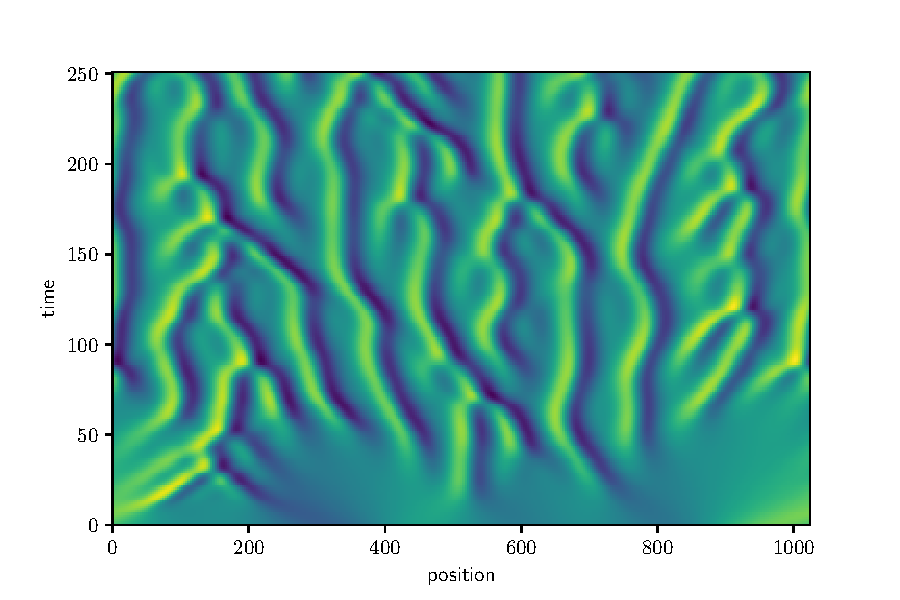
\includegraphics[width=\textwidth]{img/sample_KS_trajectory.pdf}
    \caption{trajectory generated by {\tt solve\_ivp}}
    \label{sample_KS_trajectory}
\end{subfigure}\hfill
\begin{subfigure}{.45\textwidth}\centering
    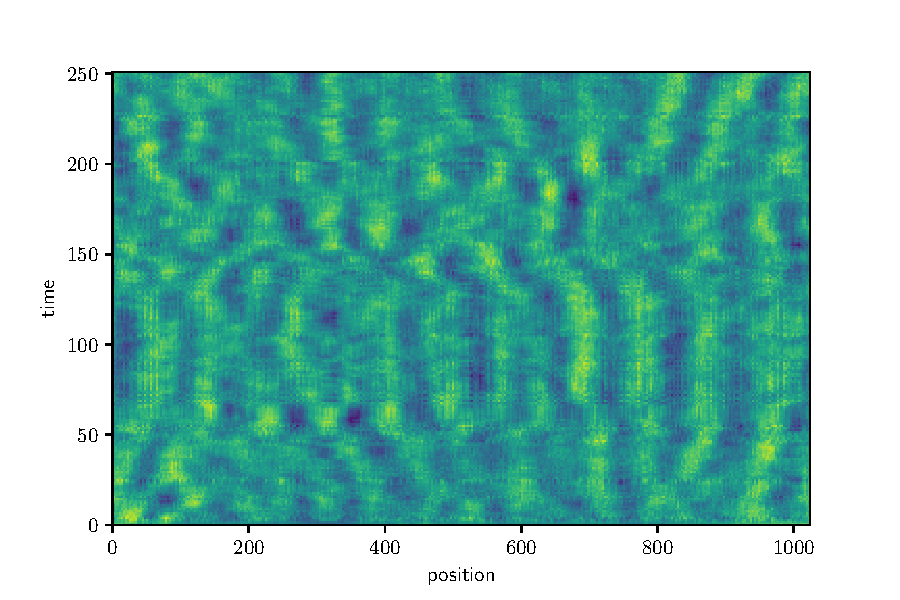
\includegraphics[width=\textwidth]{img/predicted_KS_trajectory.pdf}
    \caption{trajectory generated by neural net}
    \label{predicted_KS_trajectory}
\end{subfigure}
\caption{``actual'' and neural net predicted trajectories for Kuramoto-Sivashinsky equation (\ref{KS_eqn})}
\label{KS_trajectory}
\end{figure*}

Figure~\ref{1mode} shows the dominant left singular vector and Figure~\ref{1coeff} shows how the first right singular vector varies in time. The ``spikes'' down clearly are related to the initial conditions of the data. However, after each spike there is an oscillation in this mode. Moreover, the mode itself has quite a bit of structure, which it seems to have inherited from the way we generated initial conditions. It is not clear whether this structure would die out if we ran the simulations for longer time. Regardless, since the structure is present in our data set we can use this to train a neural net on the rank-reduced data.

We take the rank \( k \) SVD (\ref{SVD_eq}) (determined by a parameter flag) and then train the network on the weights of the basis of the subspace spanned by the first \( k \) columns of \( U \).

To test our prediction we take a trajectory not used for training, project it to the column span of \( U \), iteratively apply the network, and then embed back to the original space.


\subsection{Lorenz Equation}
The Lorenz equation (\ref{lorenz_eq}) is a system of ODEs which have chaotic solutions for some parameters. It was demonstrated in \cite{lecture_notes} that for a fixed \( \Delta t \) a simple neural network can be trained to predict the position at a time \( t+\Delta t \) given the position at time \( t \) accurately enough that the trajectory determined by iteratively applying the trained neural net matches the trajectory of a given ODE solver almost exactly. Given that the system is chaotic for these values it is somewhat surprising that the neural net manages to follow the same trajectory by only predicting one step at a time. Training data was generating using Scipy's {\tt solve\_ivp} with a tolerance of \( 10^{-10} \) and evaluating the solution along a mesh of uniformly spaced times.

\begin{align}
    \pp{}{t} \left[\begin{array}{c}x\\y\\z\end{array}\right]
    =
    \left[\begin{array}{c}
        \sigma(y-x) \\
        x (\rho-z)-y \\
        x y-\beta z
    \end{array}\right] \label{lorenz_eq}
\end{align}

We explore the Lorenz equation in two further ways, namely trying to predict trajectories for varying values of the parameter \( \rho \) and trying to predict when the solution will transition from one lobe to another.

The first task is straightforward. In particular, a neural net is trained on data where the input corresponds to the current position as well as the value of \( \rho \), and the output is the position after a time of \( \Delta t \). More specifically, we fix \( \sigma = 10 \), \( \beta = 8/3 \), and train on data with \( \rho = 10,28,40 \). We then try to use this net to predict trajectories for \( \rho = 17 \) and \( \rho = 35 \).

The second tasks requires some interpretation. We decided to train a network to determine how long until a lobe switch. To train such a network requires that we know how long it will be until the solution switches lobes. To do this we first classify what it means to be at a given lobe. This is done by separating the data with plane as shown in Figure~\ref{separating_hyperplane}. Let \( c \) be a normal vector for this hyperplane. Then the sign of \( c^Tx \) will determine which side of the plane a given point is on.

We pick \( c \) roughly in the direction of the vector connecting the two centers in the \( x \)-\( y \) plane. While there are probably better ways to do this, it seems like the projection to this plane provides a straightforward way to separate points circle different lobes.

Therefore, given a trajectory \( X \), each point in the trajectory can be classified as ``left'' or ``right''. Once this is done, we know that transitions across the plane occur when the trajectory switches from ``left'' to ``right'' or from ``right'' to ``left''. We compute these transition points by taking the difference of consecutive points in \( \operatorname{sign}(c^TX) \). If the difference is nonzero then the trajectory has switched lobes. Once we have these transition points it is relatively straightforward label each point in the trajectory with far each point is from the next crossover.

As a minor note, some of the data from the end of the each trajectory is discarded because it is not possible to tell when the next transition will occur without stepping out the solution further. We then train a neural network to try and predict the time until a crossover.
\begin{figure}[tb!]\centering
\begin{subfigure}{.45\textwidth}\centering
    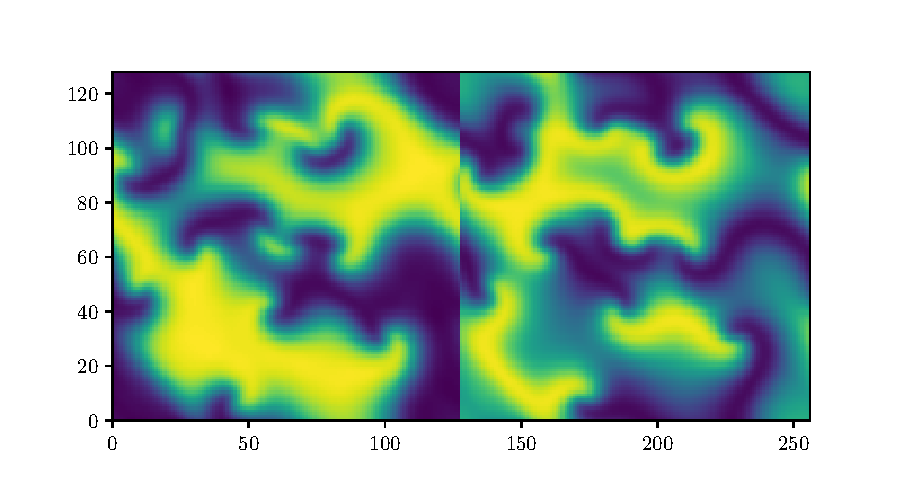
\includegraphics[width=\textwidth]{img/uv_t180.pdf}
    \caption{original data}
    \label{time_image}
\end{subfigure}\hfill
\begin{subfigure}{.45\textwidth}\centering
    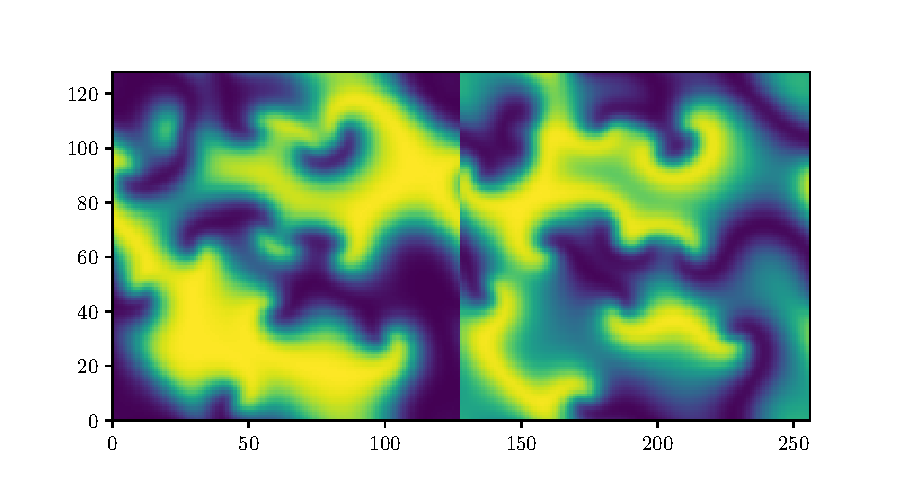
\includegraphics[width=\textwidth]{img/svd_t180.pdf}
    \caption{SVD (rank 100)}
    \label{SVD_time_image}
\end{subfigure}
\caption{snapshot of \( u \) (left) and \( v \) (right) at time \( t=180 \)}
\label{RD_SVD}
\end{figure}

\begin{figure}[b!]\centering
\begin{subfigure}{.45\textwidth}\centering
    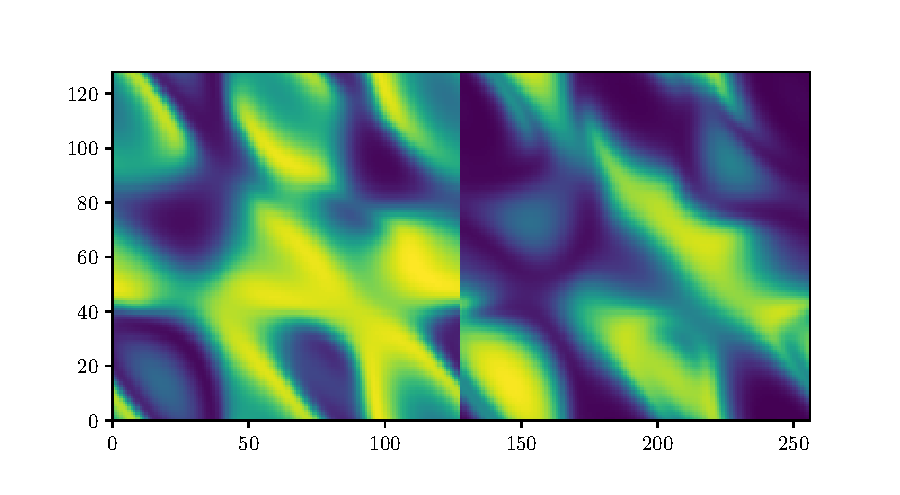
\includegraphics[width=\textwidth]{img/prediction_t15.pdf}
    \caption{actual trajectory}
    \label{sample_RD_trajectory}
\end{subfigure}\hfill
\begin{subfigure}{.45\textwidth}\centering
    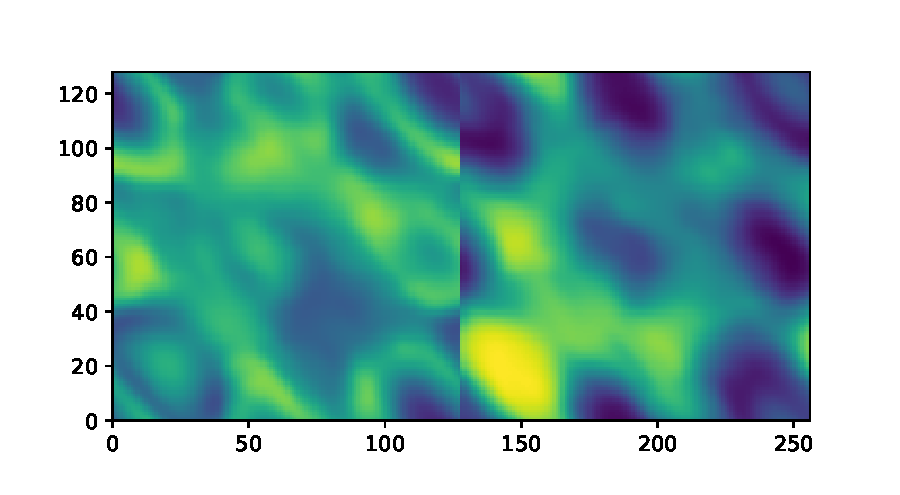
\includegraphics[width=\textwidth]{img/svd_prediction_t15.pdf}
    \caption{predicted trajectory}
    \label{predicted_RD_trajectory}
\end{subfigure}
\caption{``actual'' and neural net predicted trajectories for Reaction Diffusion Equation (\ref{RD_eqn}) at \( t=15 \)}
\label{RD_trajectory}
\end{figure}

\begin{figure}[t!]\centering
\begin{subfigure}{.45\textwidth}\centering
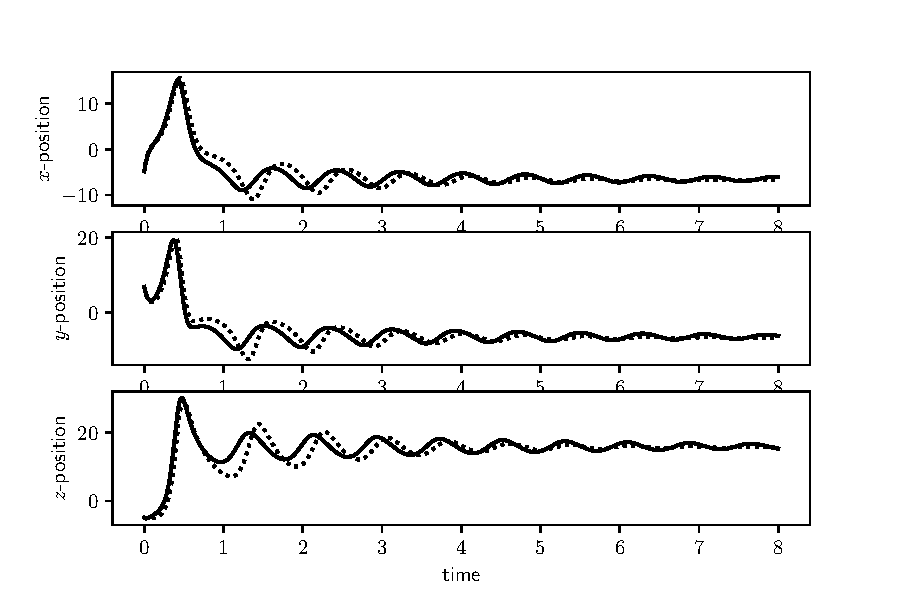
\includegraphics[width=\textwidth]{img/NN_lrz17_trajectory.pdf}
\caption{\( \rho = 17 \)}
\end{subfigure}\hfill
\begin{subfigure}{.45\textwidth}\centering
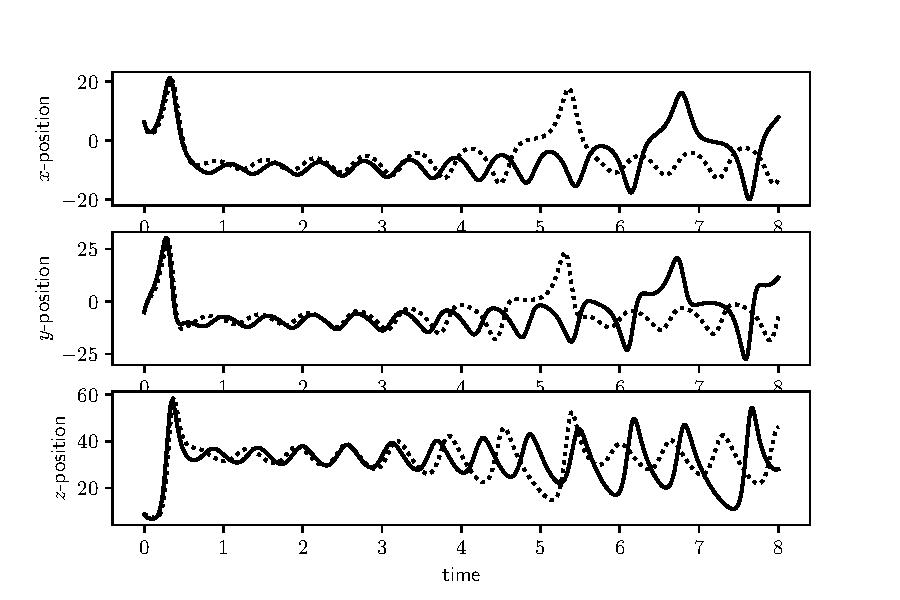
\includegraphics[width=\textwidth]{img/NN_lrz35_trajectory.pdf} \hfill
\caption{\( \rho = 35 \)}
\end{subfigure}
\caption{Actual trajectory (solid) vs predicted trajectory (dotted) for variious values of \( \rho \)}
\label{xyz_trajectory}
\end{figure}




\section{Computational Results}

\subsection{Kuramoto-Sivashinsky Equation}

Figure~\ref{sample_KS_trajectory} shows a sample trajectory generated by our ODE stepper (not part of traninig data). Figure~\ref{predicted_KS_trajectory} shows the prediction of the neural net on the same trajectory. However, as time progresses the neural net predicted solution does not really change, while the reaction diffusion equation does continue to evolve.


\subsection{ \( \boldsymbol\lambda \)-\( \boldsymbol\omega \) Reaction-Diffusion Equation}
Figure~\ref{time_image} shows a snaptshot of a trajectory at time \( t=180 \). Figure~\ref{SVD_time_image} shows the same snapshot after it has been projected into a 100 dimensional subspace determined by the SVD. While a plot of the singular values shows no clear cutoff in the rank, visually it seems that the data is fairly well represented by the first 100 modes. We proceed to train a neural network on the rank reduced data.

\begin{figure}[bt!]\centering
\begin{subfigure}{.45\textwidth}\centering
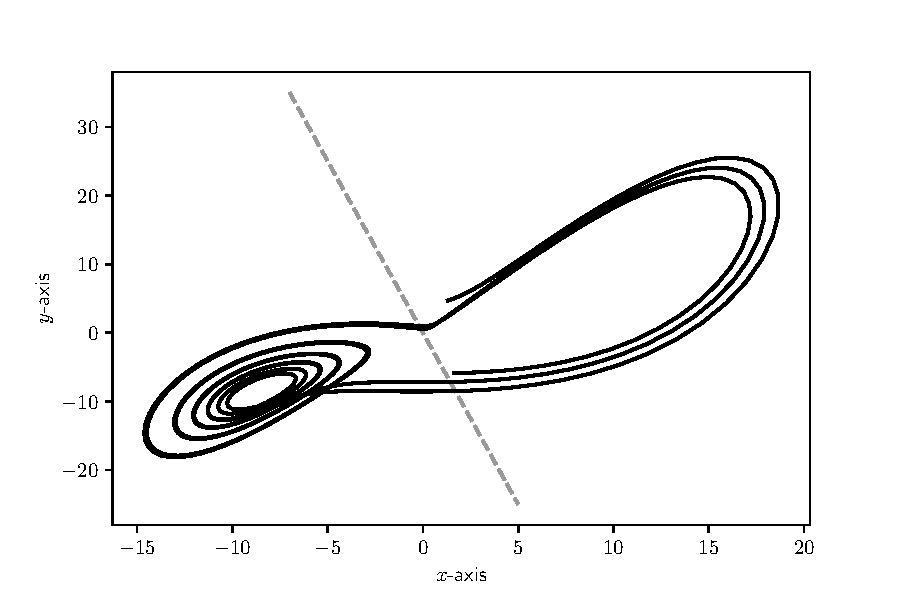
\includegraphics[width=\textwidth]{img/separating_hyerplane.pdf}
\caption{Projection of sample trajectory onto the \( x \)-\( y \) plane along with image of plane \( y + 5x +0z = 0 \).}
\label{separating_hyperplane}
\end{subfigure}\hfill
\begin{subfigure}{.45\textwidth}\centering
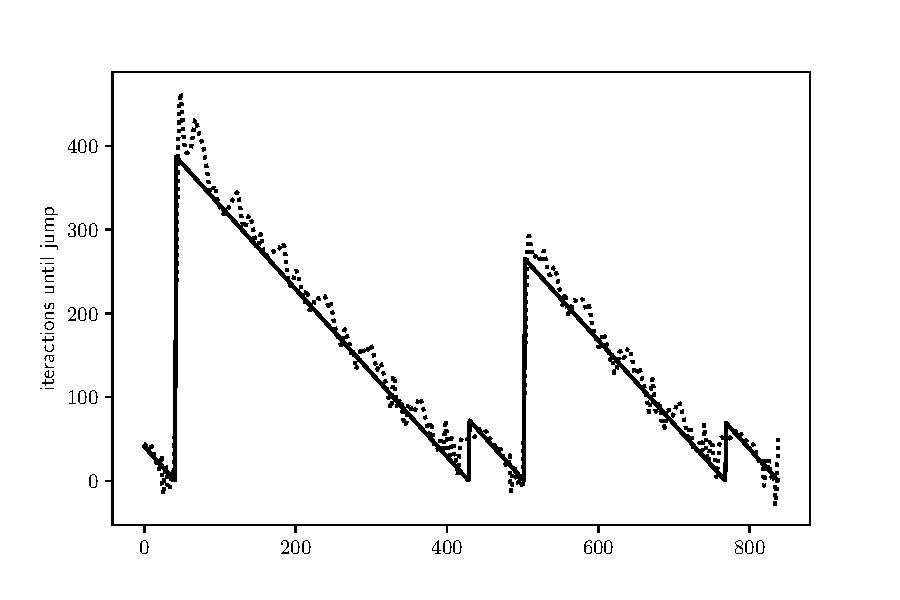
\includegraphics[width=\textwidth]{img/jump_predictor.pdf}
\caption{Actual time to jump (solid) vs. predicted time to jump (dotted) for sample trajectory .}
\label{jump_predictor}
\end{subfigure}
\caption{}
\end{figure}

\subsection{Lorenz Equation}
Sample predictions for \( \rho = 17 \) and \( \rho = 35 \) produced by the trained net are shown in Figure~\ref{xyz_trajectory}. Note that we do not cross validate in the normal sense, since that would be testing how well our net can predict one step in the future. In fact, the cross validation would show a very high accuracy since we are able to predict the long term behavior relatively well despite only training n the current position.

Figure~\ref{jump_predictor} shows the results of applying the trained net to every point in a trajectory. This plot makes it clear that we are actually able to fairly effectively determine when a jump will occur given only the current position. Note here that the horizontal axis labeling is just the index of the point in the trajectory and has no impact on the neural net's prediction as it is applied independently to each point.

\pagebreak
\section{Summary and Conclusions}
It is clear that the trajectories of the Kuramoto-Sivashinsky and Reaction Difussion equations were not effectively predicted. On the other hand, solutions to the Lorenz equation, even for values of \( \rho \) which the neural net had never seen, were quite successful. Finally, we were able to train a neural net to predict how long it would take a trajectory to switch lobes.

Due to time constraints only simple nets were used and all hyperparameter training was done by guessing. We instead chose to focus on producing the training data in a scalable way so that in the future it would be a trivial task to generate data at large mesh sizes. With the current state of our codebase, testing new neural nets is as easy as changing a few lines in Keras. Given more time we would have liked to set up convolutional neural nets to see if the local structure of the data would be enough to determine the global behavior. In general we probably did not use enough data, and the nets we used are probably too small to be able to get very good results. However, what we did find is somewhat encouraging and given more time would be worth pursuing.


\bibliographystyle{plain}
\bibliography{hw2}

\onecolumn
\section{Appendix A}
\label{AppendixA}
All functions are included in the code in Appendix B as they are specific to the task performed in each of the files.

%\pagebreak
\section{Appendix B}
\lstinputlisting[]{PDECODES/KS_data_gen.m}
\lstinputlisting[]{python/hw2_ks.py}
\lstinputlisting[]{PDECODES/RD_data_gen.m}
\lstinputlisting[]{python/hw2_rd.py}
\lstinputlisting[]{python/hw2_lrz.py}
\lstinputlisting[]{python/lrz_classifier.py}


\end{document}
